\section{2D \texorpdfstring{$U(1)$}{U (1)} Lattice Gauge Theory}%
\label{sec:l2hmc_u1} 
All lattice QCD simulations are performed at finite
lattice spacing $a$ and need an extrapolation to the continuum in order to be
used for computing values of physical quantities.
%
More reliable extrapolations can be done by simulating the theory at
increasingly smaller lattice spacings.
%
The picture that results when the lattice spacing is reduced and the physics
kept constant is that all finite physical quantities of negative mass dimension
diverge if measured in lattice units.
%
In statistical mechanics language, this states that the continuum limit is a
critical point of the theory since correlation lengths diverge.
%
MCMC algorithms are known to encounter difficulties when used for simulating
theories close to a critical point, an issue known as the \emph{critical slowing
down} of the algorithm.
%
This effect is most prominent in the topological charge, whose auto-correlation
time increases dramatically with finer lattice spacings.
%
As a result, there is a growing interest in developing new sampling techniques
for generating equilibrium configurations. 
%
In particular, algorithms that are able to offer improvements in efficiency
through a reduction of statistical autocorrelations are highly desired. 
%
We begin with the two-dimensional $U{(1)}$ lattice gauge theory with dynamical
variables $U_{\mu}{(i)}$ defined on the links of a lattice, where $i$ labels a
site and $\mu$ specifies the direction.
%
Each link $U_{\mu}{(i)}$ can be expressed in terms of an angle $0 <
\phi_{\mu}{(i)} \leq 2 \pi$.
%
\begin{equation}
    U_{\mu}{(i)} = e^{i\phi_{\mu}{(i)}}
    \label{eq:link_variable}
\end{equation}
%
with the Wilson action defined as:
%
\begin{equation}
    \beta S = \beta \sum_{P}{(1 - \cos{(\phi_{P})})}
    \label{eq:wilson_action}
\end{equation}
%
where
%
\begin{equation}
    \phi_{P} \equiv \phi_{\mu\nu}(i) = 
        \phi_{\mu}{(i)} + \phi_{\nu}{(i + \hat{\mu})} 
        - \phi_{\mu}{(i + \hat{\nu})} - \phi_{\nu}{(i)}
    \label{eq:phi_plaquette}
\end{equation}
%theta_
and $\beta = 1/e^{2}$ is the gauge coupling, and the sum $\sum_{P}$ runs over
all plaquettes of the lattice.
%
An illustration showing how these variables are defined for an elementary
plaquette is shown in Fig.~\ref{fig:plaquette}.
%
\begin{figure}[htpb]
  \centering
  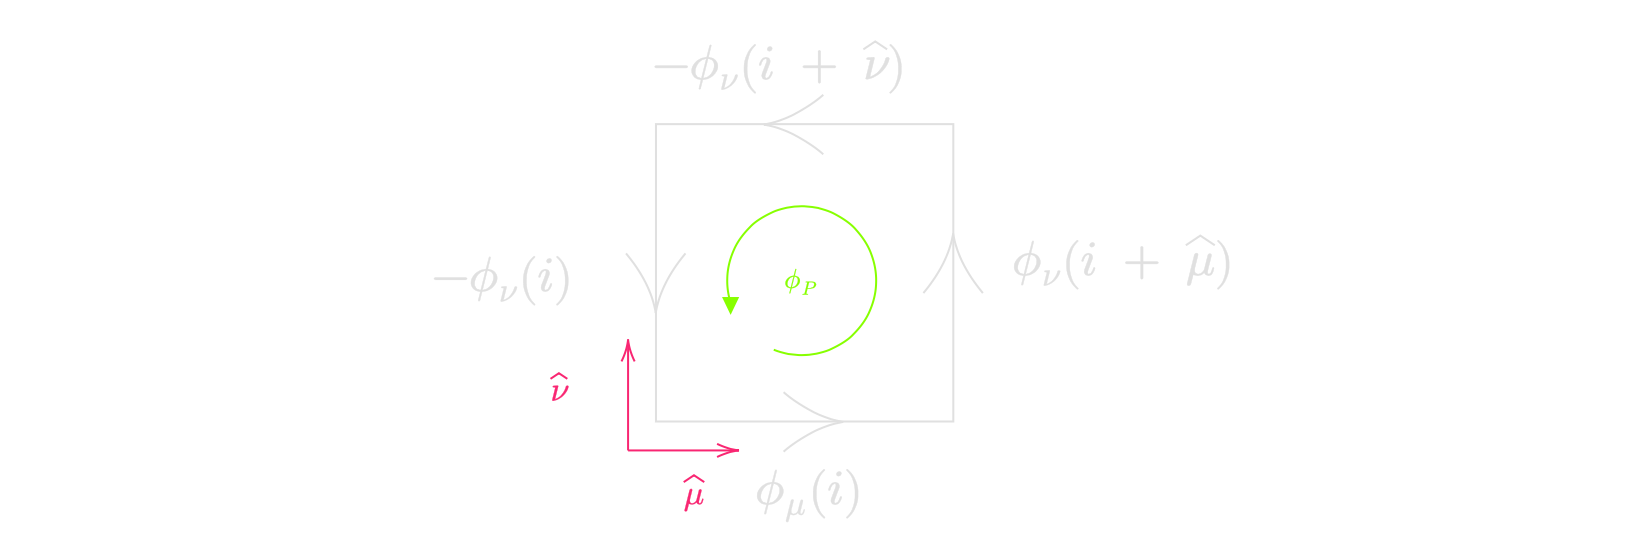
\includegraphics[width=0.5\textwidth]{gauge_figures/plaq.png}
  \caption{Illustration of an elementary plaquette on the lattice.}%
\label{fig:plaquette}
\end{figure}

We can define the topological charge, $\mathcal{Q} \in \mathbb{Z}$, as
%
\begin{equation}
  \mathcal{Q} \equiv \frac{1}{2\pi}\sum_{P} \tilde \phi_{P} =
    \frac{1}{2\pi}\sum_{\substack{{i; \mu, \nu}\\{\nu > \mu}}}
    \tilde \phi_{\mu\nu}{(i)}
    \label{eq:topological_charge}
\end{equation}
%
where
%
\begin{equation}
  \tilde{\phi}_{P} \equiv \phi_{P} - 2\pi {\bigg\lfloor{\frac{\phi_{P} +
  \pi}{2\pi}\bigg\rfloor}}
  % \tilde{\phi}_{P} \equiv \phi_{P} - 2 \pi \left \lfloor{\frac{\phi_{P} +
  % \pi}{2 \pi}\right \rfloor}
\end{equation}
%
is the sum of the link variables around the elementary plaquette, projected
onto the interval $\left[0, 2 \pi\right)$.
%
From this, we can define topological susceptibility
%
\begin{equation}
    \chi \equiv \frac{\langle \mathcal{Q}^2\rangle - \langle \mathcal{Q} \rangle^2}{V}
    % \label{eq:topological_susceptibility}
\end{equation}
%
By parity symmetry, $\langle \mathcal{Q} \rangle = 0$, so we have that
\begin{equation}
    \chi = \frac{\langle \mathcal{Q}^2\rangle}{V}
    \label{eq:topological_susceptibility}
\end{equation}
%
Unfortunately, the measurement of $\chi$ is often difficult due to the fact
that the autocorrelation time with respect to $\mathcal{Q}$ tends to be extremely long.
%
This is a consequence of the fact that the Markov chain tends to get stuck in a
topological sector (characterized by $\mathcal{Q} = const$.), a phenomenon known as
\emph{topological freezing}.
%
% (right) Topological charge vs.\ step generated using the trained
% L2HMC sampler.}%
\begin{figure}[htpb]
  \centering
    % \includegraphics[width=0.49\textwidth]{top_charge_vs_step_hmc.eps}
    % \includegraphics[width=0.49\textwidth]{top_charge_vs_step_l2hmc.eps}
    \includegraphics[width=0.6\textwidth]{charge_plots/top_charge_vs_step_HMC}
    % \includegraphics[width=0.49\textwidth]{charge_plots/compare/top_charge_vs_step_hmc}
    % \includegraphics[width=0.49\textwidth]{charge_plots/compare/top_charge_vs_step_l2hmc}
    \caption{Example of topological freezing in the $2D$ $U{(1)}$
      lattice gauge theory. The above result was generated using generic HMC
      sampling for a $8\times8$ lattice. Note that for the majority of the
      simulation $\mathcal{Q}=0$, making it virtually impossible to get a reasonable
    estimate of $\chi$.}\label{fig:top_charge} 
  \end{figure}
%
%
%%%%%%%%%%%%%%%%%%%%%%%%%%%%%%%%%%%%%%%%%%%%%%%%%%%%%%%%%%%%%%%%%%%%%%%%%%%%%%%
\subsection{Annealing Schedule}% 
\label{subsec:l2hmc_u1annealing}
% In addition to modifying the neural network architecture, we also modified
% the training algorithm to follow a simulated annealing schedule.
%
Proceeding as in the example of the Gaussian Mixture Model, we include a
simulated annealing schedule in which the value of the gauge coupling $\beta$
is continuously updated according to the annealing schedule shown in
Eq.~\ref{eq:annealing_schedule}.
%
% Explicitly, the value of the gauge coupling $\beta$ is continuously updated
% according to the annealing schedule shown in Eq.~\ref{eq:annealing_schedule}.
%
This was done in order to encourage sampling from multiple different
topological charge sectors, since our sampler is less `restricted' at lower
values of $\beta$.
%This was don
\begin{equation} 
  \frac{1}{\beta(n)} = {\left(\frac{1}{\beta_{i}} 
    - \frac{1}{\beta_{f}}\right)}
    {\left(\frac{1 - n}{N_{\mathrm{train}}}\right)} 
    + \frac{1}{\beta_{f}} 
\label{eq:annealing_schedule} 
\end{equation}
%
Here $\beta(n)$ denotes the value of $\beta$ to be used for the
$n^{\mathrm{th}}$ training step ($n = 1, \ldots, N_{\mathrm{train}}$),
$\beta_{i}$ represents the initial value of $\beta$ at the beginning of the
training, and $\beta_{f}$ represents the final value of $\beta$ at the end of
training.
%
For a typical training session, $N_{\mathrm{train}} = 25,000$, $\beta_{i} = 2$
and $\beta_{f} = 5$.
% For all of the exmaples above, $N_{\mathrm{train}} = 25,000$, $\beta_{0} = 2$
% and $\beta_{N_{\mathrm{train}}} = 5$.
%
% As can be seen in Fig.~\ref{fig:top_charge}

\subsection{Modified metric for \texorpdfstring{$U(1)$}{U (1)} Gauge
Model}%
\label{subsec:l2hmc_modifiedloss}
%
In order to more accurately define the ``distance'' between two different
lattice configurations, we redefine the metric in Eq.~\ref{eq:metric_orig} to
be
%
\begin{equation}
  % \delta(\xi(\phi_{\mu}(x)), \xip(\phi_{\mu}(x))) \equiv 1 -
  % \cos\left(\xi(\phi_{\mu}(x)) - \xi^{\prime}(\phi_{\mu}(x))\right)
  \delta(\xi, \xip) \equiv 1 - \cos\left(\xi - \xi^{\prime}\right)
\label{eq:new_metric}
\end{equation}
%
where now $\xi \equiv {\left(\phi_{\mu}^{x}(i), \,\phi_{\mu}^{v}(i),\,
d\right)}$, with $\phi_{\mu}^{x}$ representing the lattice of (`position')
gauge variables (what we called $x$ previously), and $\phi_{\mu}^{v}$
representing the lattice of (`momentum') gauge variables (what we called $v$
previously). Note that $i$ runs over all lattice sites\footnote{In what
  follows, we will refrain from explicitly including the site index and make
  the assumption that it implicitly extends over all sites on the lattice.} and
  $\mu=0, 1$ for the two dimensional case.
%
We see that this metric gives the expected behavior, since $\delta \rightarrow
0$ for $\xi \approx \xip$.

%%%%%%%%%%%%%%%%%%%%%%%%%%%%%%%%%%%%%%%%%%%%%%%%%%%%%%%%%%%%%%%%%%%%%%%%%%%%%%%
%
%%%%%%%%%%%%%%%%%%%%%%%%%%%%%%%%%%%%%%%%%%%%%%%%%%%%%%%%%%%%%%%%%%%%%%%%%%%%%%%
% \subsection{Issues with the Average Plaquette}
% %
% When running inference using the trained sampler, an issue was encountered in
% which the average plaquette, $\langle \phi_{P}\rangle$ seems to converge to a
% value which is noticeably different from the expected value in the infinite
% volume limit, and can be seen in Fig.~\ref{fig:bad_convergence}.
% %
% In order to quantify this unexpected behavior, we can calculate the difference
% between the observed value of the average plaquette, $\langle \phi_{P}\rangle$
% and the expected value $\phi_{P}^{(*)}$ (calculated from the infinite volume
% limit):
% %
% \begin{equation}
%   {\delta_{\phi_P}}(\alpha_Q, N_{\mathrm{LF}}) \equiv \langle \phi_P\rangle -
%   \phi_{P}^{(*)} \neq 0.
%   % - \langle{\phi_{P}^{\mathrm{(exact)}}}\rangle \neq 0}.
% \end{equation}
% %
% % Which allows us to quantify this difference.%
%
%
% % Upon further testing, an issue was encountered in which the
% % of the average plaquette
% % $\langle \phi_{P}\rangle$ seems to converge to a value which is noticeably
% % different from the expected value in the infinite volume limit.
% %
% % This behavior can be seen in Fig.~\ref{fig:bad_convergence}, and seems to
% % depend on both the number of augmented leapfrog steps used by our integrator,
% % as well as the `strength' of the topological loss term in
% % Eq.~\ref{eq:topological_loss_term}.
% %
% % The parameters used in Fig~\ref{fig:bad_convergence} are as follows: $L = 8$,
% % $N_{\mathrm{LF}} = 7$, and $N_{\mathrm{samples}} = 128$,
% % and the sampler was trained for $N_{\mathrm{train}} = 1\times10^{4}$.
% %
% % In Fig~\ref{fig:good_convergence}, the only change was the weight factor for
% % the topological charge term in the loss function $\alpha_{Q} = 0$.
% %
% \begin{figure}[htpb]%
%   \centering
%     \includegraphics[width=0.49\textwidth]{new_figures/plaq_error/plaqs_diffs_vs_step_l2hmc_lf16.pdf}
%     \includegraphics[width=0.49\textwidth]{new_figures/plaq_error/plaqs_diffs_vs_step_hmc_lf16.pdf}
%     % \includegraphics[width=0.49\textwidth]{plaq_plots/plaqs_diffs_vs_step_bad.pdf}
%     \caption{Difference between the observed and expected value of the average
%       plaquette, $\delta_{\phi_{P}}$, \textbf{(left)}: using the trained L2HMC
%       sampler, and \textbf{(right)}: using generic HMC.}%
%       % trained L2HMC sampler \textbf{(left)} and generic HMC \textbf{(right)} .
%       % HMC result, obtained by setting $\alpha_{S} = \alpha_{Q} = \alpha{T} = 0$
%       % \textbf{(right)}:
%       % \ref{subsec:net_weights}).}%
% \label{fig:bad_convergence}
% \end{figure}%
% %%%%%%%%%%%%%%%%%%%%%%%%%%%%%%%%%%%%%%%%%%%%%%%%%%%%%%%%%%%%%%%%%%%%%%%%%%%%%%%
